% !TeX root = exam.tex
% The exam itself, shared by exam.tex (to print) and exam-solutions.tex.
% Shared by the exam and the collection: packages, macros, how solutions look.
% Course details: change them here once.
\newcommand{\coursename}{Course Name}
\newcommand{\lecturer}{Lecturer Name}
\newcommand{\institution}{University of Vienna}
\newcommand{\term}{Winter Term 2026/2027}

% question title in bold, points in brackets: "1. Title (10)"
\makeatletter
\qformat{\thequestion. \bfseries\thequestiontitle\if@placepoints~(\thepoints)\else\fi\hfill}
\makeatother

\usepackage{a4wide}
\usepackage{graphicx}
\usepackage{xcolor}
\usepackage{booktabs}
\usepackage{amsmath,amssymb,amsthm,bm}
\usepackage[hidelinks]{hyperref}

\newtheorem{theorem}{Theorem}

% solutions on a light blue background
\shadedsolutions
\definecolor{SolutionColor}{rgb}{0.9,0.95,1}
\renewcommand{\solutiontitle}{\noindent\emph{Solution}\par\nopagebreak\noindent}


\newcommand{\examtitle}{Midterm Exam}

% Each exercise starts on a new page. Parts that should start on a page of their own in the
% printed exam call \exambreak (it does nothing in the solutions, which simply run on).
\ifprintanswers\else\newcommand{\exambreak}{\newpage}\fi

% Box heights: the exercises give them as \boxheight{9} (9 cm by default, see the exercise files).
% With the next line they are shares of a page's free space instead, so the boxes fill their
% pages (two boxes of \boxheight{1} on a page get half of it each). This needs every page to
% end in \clearpage or \exambreak. Comment it out for fixed heights in cm.
\newcommand\boxheight[1]{\stretch{#1}}

\runningheader{\coursename}{}{\thepage}
\runningfooter{}{}{}

\begin{document}

\vspace{5mm}
\makebox[0.75\textwidth]{Name:\enspace\hrulefill}

\vspace{5mm}
\makebox[0.75\textwidth]{Student ID:\enspace\hrulefill}

\vfill

\begin{center}
  {\Large \examtitle}\\ \bigskip
  {\large \coursename}\\ \bigskip
  {\large \term}

  \vfill

  \begin{itemize}
    \item This exam consists of \numquestions\ problems, worth \numpoints\ points in total.
    \item Write your answers into the provided boxes.
    \item If you run out of space, use the \emph{Extra space} at the end of this exam.
    \item The exam takes 90 minutes. It is closed-book.
    \item You may use a pen, a ruler and a non-graphical calculator.
  \end{itemize}
\end{center}

\vfill

\begin{center}
  \gradetable[v][questions]
\end{center}

\clearpage

\begin{questions}
\providecommand\boxheight[1]{#1cm} % a box's height in cm, unless the exam redefines it
\titledquestion{Centrality} Consider the following network
\begin{equation*}
    G = \begin{pmatrix}
        1 & 1 & 1 \\
        1 & 1 & 1 \\
        1 & 1 & 1 \\
    \end{pmatrix}.
    \end{equation*}
Let $\beta_i = 1$ be the exogenous importance of each node.

\begin{parts}
    \part[3] Draw the network.
    \begin{solutionorbox}[\boxheight{10}]
        
        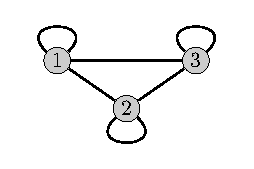
\includegraphics{centrality/centrality-simple_complete}
    \end{solutionorbox}
    \ifdefined\exambreak\exambreak\fi % an exam may start this part on a new page (its box does not fit under the part before)
    \part[7] Compute the Katz-Bonacich centrality for each node of the network for a suitable range of $\alpha$.

    \begin{solutionorbox}[\boxheight{20}]
        \begin{enumerate}
            \item   Note that 
        \begin{equation*}
            G = 3 \underbrace{\begin{pmatrix}
                \frac{1}{3} & \frac{1}{3} & \frac{1}{3} \\
                \frac{1}{3} & \frac{1}{3} & \frac{1}{3} \\
                \frac{1}{3} & \frac{1}{3} & \frac{1}{3} \\
            \end{pmatrix}}_{=: \tilde G},
        \end{equation*}
        where $\tilde G$ is of the form \begin{equation*}
            \begin{pmatrix}
                \bm \pi^T \\ \bm \pi^T \\ \bm \pi^T
            \end{pmatrix}.
        \end{equation*}
        where $\bm \pi^T \in \mathbb{R}^{1 \times n}$ is a stochastic row vector. 
        \item Thus, by the stationary-matrix theorem, $G^i = (3 \tilde G)^i = 3^i \tilde G^i = 3^i \tilde G$ for all $i \geq 1$.
        \item The Katz-Bonacich centrality is given by \begin{equation*}
            \tilde{\bm c}^{\text{KB}} = \Bigl(\sum_{i=1}^\infty \alpha^i G^i\Bigr)^T \bm \beta
        \end{equation*}
        \item The infinite sum is
        \begin{equation*}
            \sum_{i=1}^\infty \alpha^i \underbrace{G^i}_{3^i \tilde G} = \tilde G \sum_{i = 1}^\infty (3\alpha)^i = \frac{3\alpha}{1-3\alpha} \tilde G
        \end{equation*}
        if and only if $3\alpha < 1 \iff \alpha < \frac{1}{3}$. ($\alpha$ cannot be negative.) Otherwise the sum diverges to $+\infty$.
        \item We continue under the assumption that $\alpha \in (0, \frac{1}{3}$)
        \item So, 
        \begin{equation*}
            \tilde{\bm c}^{\text{KB}} = \frac{3\alpha}{1-3\alpha} \tilde G^T \bm \beta = \frac{3\alpha}{1-3\alpha} 
        \begin{pmatrix}
            \frac{1}{3} & \frac{1}{3} & \frac{1}{3} \\
            \frac{1}{3} & \frac{1}{3} & \frac{1}{3} \\
            \frac{1}{3} & \frac{1}{3} & \frac{1}{3} \\
        \end{pmatrix} \begin{pmatrix}
            1 \\ 1 \\1 
        \end{pmatrix} = \frac{3\alpha}{1-3\alpha} \begin{pmatrix}
            1 \\ 1 \\1 
        \end{pmatrix}
    \end{equation*}
       \item So $\tilde{c}^{\text{KB}}_i =  \frac{3\alpha}{1 - 3\alpha}$ for each node $i$, as long as $\alpha \in (0, \frac{1}{3}$).
    \end{enumerate}
    \end{solutionorbox}
\end{parts}
\clearpage
\providecommand\boxheight[1]{#1cm} % a box's height in cm, unless the exam redefines it
\titledquestion{Social Connectedness}
Let $X$ be the set of US counties and $x \in X$. Then the set of counties whose distance is less than $r$ can be denoted by

\begin{equation*}
    B_r(x) = \{ x' \in X : d(x, x') < r \}
\end{equation*}

The measure of network concentration is defined as

\begin{equation*}
    C_x^r = \frac{
    \sum_{y \in B_r(x)} \#_{x,y} }{\sum_{z \in X} \#_{x,z}}
\end{equation*}
where $\#_{x,y}$ is the number of friendships between counties $x$ and $y \in X$.

\begin{parts}
    \part[2] Briefly interpret the measure of network concentration.

    \begin{solutionorbox}[\boxheight{4.5}]
      $C_x^r$ is the fraction of county $x$'s friendships that are with people living within distance $r$ of $x$ (the share of $x$'s friends who live nearby).
    \end{solutionorbox}

    \part[2] State the definition of the Social Connectedness Index $\text{sci}_{x,y}$ for $x,y \in X$.

    \begin{solutionorbox}[\boxheight{7}]
      With $\#_x$ the number of Facebook users in county $x$,
      \begin{equation*}
        \text{sci}_{x,y} = \frac{\#_{x,y}}{\#_x \cdot \#_y}.
      \end{equation*}
    \end{solutionorbox}

    \ifdefined\exambreak\exambreak\fi % an exam may start this part on a new page (its box does not fit under the part before)
    \part[4] Rewrite $C_x^r$ in terms of the Social Connectedness Index and the population $\text{pop}_{x}$ for $x \in X$.

    \begin{solutionorbox}[\boxheight{10.5}]
      By (b), $\#_{x,y} = \text{sci}_{x,y} \, \#_x \#_y$. The factor $\#_x$ cancels:
      \begin{equation*}
        C_x^r = \frac{\sum_{y \in B_r(x)} \text{sci}_{x,y} \, \#_x \#_y}{\sum_{z \in X} \text{sci}_{x,z} \, \#_x \#_z}
              = \frac{\sum_{y \in B_r(x)} \text{sci}_{x,y} \, \#_y}{\sum_{z \in X} \text{sci}_{x,z} \, \#_z}
              \approx \frac{\sum_{y \in B_r(x)} \text{sci}_{x,y} \, \text{pop}_y}{\sum_{z \in X} \text{sci}_{x,z} \, \text{pop}_z},
      \end{equation*}
      where the last step assumes that the same fraction of each county's population uses Facebook, $\#_y = \kappa \, \text{pop}_y$ ($\kappa$ cancels).
    \end{solutionorbox}

    \part[2] Briefly describe one strength and one weakness of the Facebook Social Connectedness Index.

    \begin{solutionorbox}[\boxheight{7}]
      e.g.\
      \begin{itemize}
        \item (+): available on a very disaggregated level, for most regions of the world
        \item (-): not available for China, not reliable for Russia
        \item (-): Facebook friendships are an imperfect measure of actual friendships
      \end{itemize}
    \end{solutionorbox}
\end{parts}


\clearpage

\textbf{\emph{Extra space}}

\begin{solutionorbox}[\boxheight{1}]
\end{solutionorbox}

\end{questions}

\end{document}
